\section{Motor-Modell}

Das Motormodell besteht aus den drei Baugruppen Spannungs-Strom-Wandler, Gleichstrommotor und Getriebe. Die Modellierung der Baugruppen basiert auf den in Franke \cite{franke} erstmalig aufgestellten Gleichungen, die auch in den nachfolgenden Arbeiten zum Versuchsstand weiterhin angewendet wurden. Das Modell des Gleichstrommotors wird im Rahmen der vorliegenden Arbeit nun zusätzlich um die Berücksichtigung der Selbstinduktion des Motors erweitert.

Im Folgenden wird auf die mathematische Modellierung der drei Baugruppen näher eingegangen.

\subsection{Spannungs-Strom-Wandler}

Beim am Versuchsstand eingesetzten Spannungs-Strom-Wandler handelt es sich um einen Servoverstärker, der ursprünglich zur Drehzahlregelung von Gleichstrommotoren vorgesehen ist. Entsprechend folgt der pulsweitenmoduliert arbeitende Verstärker dem Prinzip einer übergeordneten Drehzahlregelung mit unterlagerter Stromregelung. Für die Anwendung am Versuchsstand ist der übergeordnete Drehzahlregelkreis jedoch aufgetrennt und in einen Spannungs-Strom-Wandler umfunktioniert worden. Dieser dient der Vorgabe eines konstanten Stromes durch Pulsweitenmodulation der Zwischenkreisspannung am Ausgang des Wandlers proportional zur Steuerspannung am Eingang. Das stationäre Verhalten kann aus diesem Grund durch einen Proportionalitätsfaktor $K_{UI}$ beschrieben werden
	\[
	I_{Motor} = K_{UI} \cdot U_{Steuer} .
\]

Gemäß Franke \cite{franke} lässt sich die Dynamik des Wandlers durch ein $PT_1$-Glied modellieren, sodass sich für den Wandler im Laplace-Bereich insgesamt die Gleichung
	\[
	I_{Motor}(s) = \frac{K_{UI}}{1+T_{UI}s} \cdot U_{Steuer}(s)
	\]
ergibt.


\subsection{Gleichstrommotor}

Bei dem verwendeten Motor handelt es sich um eine fremderregte Gleichstrommaschine, wobei die magnetische Erregung durch einen Permanentmagneten erzeugt wird \cite{franke}. Das elektromagnetische Drehmoment des Gleichstrommotors ist näherungsweise proportional zum Ankerstrom \cite{binder}. Hierbei wird vorausgesetzt, dass keine magnetische Sättigung vorliegt.
\[
	M_e = K_I \cdot I_a
\]

Neben dem elektromagnetischen Drehmoment sind außerdem parasitäre Reibmomente zu berücksichtigen. Die Modellierung der Reibung von Motor und Getriebe wird zusammen mit der Schlittenreibung in Kapitel \ref{sec:spdModell} behandelt. Ein rückwirkendes Moment durch die Federkraft des Riemens wird auf Grund der Annahme unendlicher Riemensteifigkeit vernachlässigt. 

Weiterhin wird das Drehmoment durch die Selbstinduktion des Motors geschwächt. Dieser Effekt ist in den Motormodellen von Franke \cite{franke} und den Nachfolgearbeiten bisher nicht berücksichtigt worden. Da die Erfahrung am realen Versuchsstand jedoch gezeigt hat, dass eine Modellierung der Selbstinduktion sinnvoll erscheint, wird diese im Rahmen dieser Arbeit in das Motormodell integriert.

Zum besseren Verständnis des Effekts wird zunächst das physikalische Prinzip der Selbstinduktion bzw. Gegeninduktion vergegenwärtigt. Fließt ein Strom durch den im Magnetfeld der Permanentmagneten ruhenden Anker des Motors, wirkt senkrecht zur Stromrichtung und zur Richtung des Magnetfeldes die Lorenzkraft auf die im Leiter der Ankerwicklung befindlichen Ladungsträger (Drei-Finger-Regel bzw. Rechte-Hand-Regel in technischer Stromrichtung). Es entsteht ein Drehmoment auf die Wicklung und der Anker beginnt sich zu drehen. Durch die Drehung bewegen sich die Ladungsträger nun zusätzlich zur Stromrichtung auch in Drehrichtung des Ankers. Auf diese Bewegungskomponente kann erneut das Prinzip der Lorentzkraft angewendet werden. Die resultierende zusätzliche Kraftkomponente, die in Abhängigkeit der Drehgeschwindigkeit auf die Ladungsträger wirkt, zeigt nun gegen die Stromrichtung (Lenzsche Regel). Auf Grund der Proportionalität zum Ankerstrom, wird das Drehmoment dadurch reduziert. 

Am Versuchsstand wird dieser induzierte Gegenstrom bei geringen Winkelgeschwindigkeiten des Motors durch den Stromregler des Spannungs-Strom-Wandlers ausgeregelt. Ab einer bestimmten Winkelgeschwindigkeit und einem konstantem Sollstrom ist der induzierte Gegenstrom größer als die Stellstromreserve, sodass er nicht mehr ausgeregelt werden kann. Nun nimmt der Strom und damit das Drehmoment mit steigender Winkelgeschwindigkeit ab bis die Leerlaufdrehzahl erreicht ist. 

ABBILDUNG I(w)-Kennlinie

Auf Grund der im Wandler integrierten Strombegrenzung zum Schutz von Motor und Verstärker ist der Stellstrom der Reglers zusätzlich begrenzt. Es wird im Rahmen dieser Arbeit idealisierend angenommen, dass der begrenzte Maximalstrom des Wandlers konstant gestellt werden kann bis zum Schnittpunkt mit der Stromkennlinie der Gegeninduktion. An dieser Stelle tritt ein "`Knick"' im von der Winkelgeschwindigkeit abhängigen Stromverlauf auf. Damit wird für die Modellierung vereinfachend angenommen, dass der Regler von der Strombegrenzung nicht betroffen ist und den Begrenzungsstrom noch bis zum "`Knick"' ausregeln kann.

ABBILDUNG Ersatzschaltbild-Gleichstrommotor

Die zu modellierende Kennlinie wird bis zur 

\subsection{Getriebe}

\begin{figure}[htbp]
	\centering
		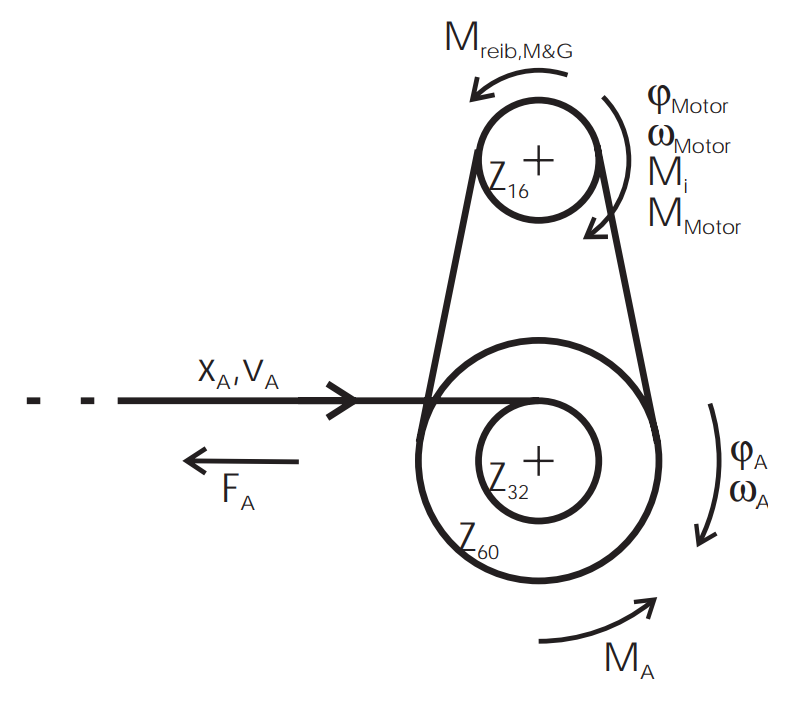
\includegraphics[width=0.50\textwidth]{Bilder/Modellierung/Getriebe.PNG}
	\caption{Getriebe \cite{franke}}
	\label{fig:Getriebe}
\end{figure}

Die Rotorbewegung des Motors wird über das in Abbildung \ref{fig:Getriebe} dargestellte Getriebe und das Antriebszahnrad auf den Zahnriemen weitergegeben. Auf Grund der hohen Steifigkeit des mit eingebetteten Stahlseilen unterstützten Riemens wird dieser wie in Apprich \cite{apprich} als unendlich starr angenommen, sodass die Verbindung von Motor und Schlitten ohne Federkopplung durch eine Übersetzungskonstante modelliert werden kann.
\[
	\dot{x} = K_G \cdot \omega_{Motor}
\]
 Die Übersetzungskonstante $K_G$ zwischen der Winkelgeschwindigkeit des Motors und der Schlittengeschwindigkeit wird über das Zahnverhältnis und den Antriebsradius berechnet.
\[
	K_G =  \frac{Z_{16}}{Z_{60}} \cdot r_{32} .
\]
Der Antriebsradius $r_{32}$ ist dabei der Abstand zwischen der neutralen Phase des Riemens und der Drehachse.